%!TEX root = ../report.tex

\section{Software Defined Networking}
Traditional networking has the problem that distributed connectivity algorithms do often times not find the best solution (e.g. spanning tree protocol) and scenario-specific requirements are generally hard to implement.
Furthermore due to the lack of abstraction, it is hard to manage a network and the innovation is slow.
Theses problems are tried to be solved by software defined networking.\\
\vspace{5pt}

The idea behind SDN is to have the control plan logically separated from the forwarding plane so that is handled centrally.
This way, the central control point can be used to calculate spanning trees or load balancing and thus render worse distributed algorithms unnecessary.
Furthermore the forwarding behavior can be specified more precisely, e.g.\ forbidding traffic from one VM to another and an higher level of abstraction can be introduced by adding a API level between hardware devices and control plane.
This abstraction greatly increases the speed in which the forwarding logic can be modified since instead of having to buy new hardware that all speak the same protocol, only some software changes have to be made.
The actual forwarding plan then only executes the specified behavior of the control plane.
Figure~\ref{fig:sdn_big_picture} shows the model of SDN.
\begin{figure}[h]
  \centering
  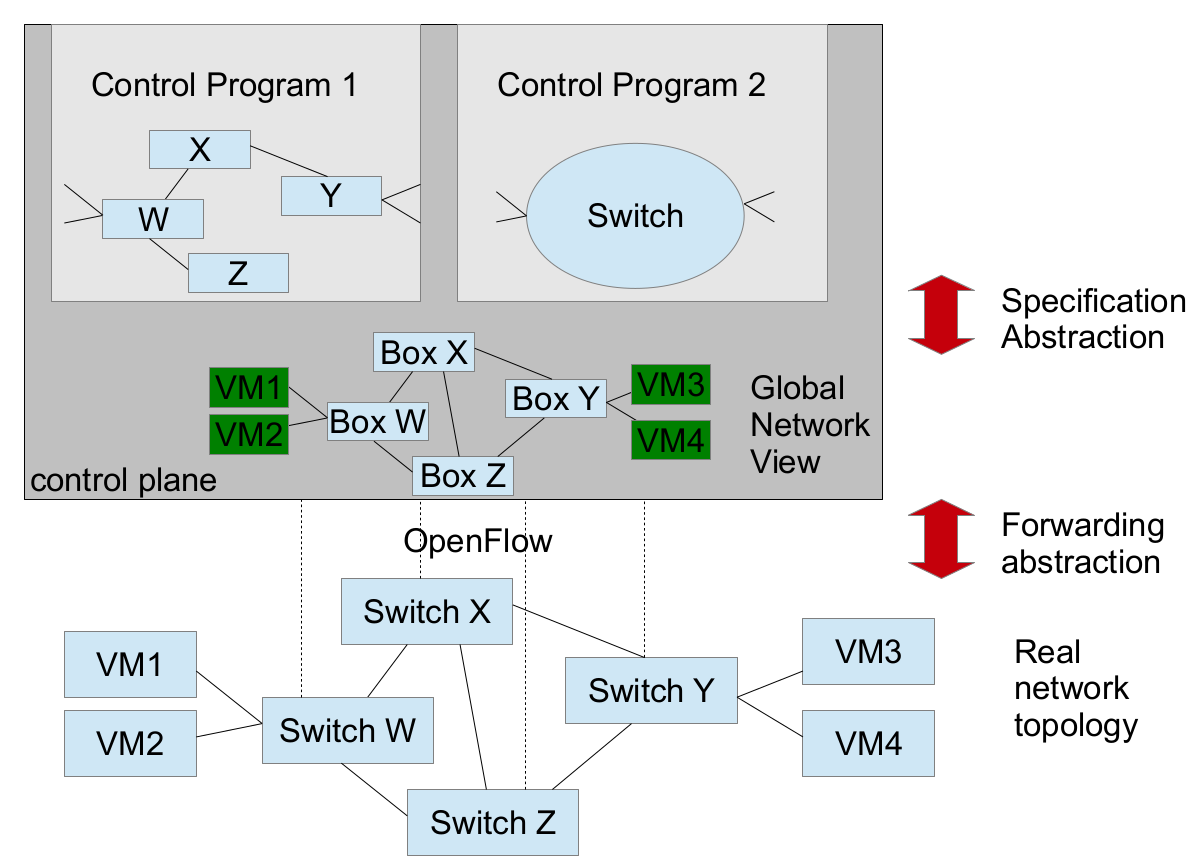
\includegraphics[width=.6\textwidth]{figures/sdn_big_picture.png}
  \caption{SDN big picture}\label{fig:sdn_big_picture}
\end{figure}

\subsection{Network Operating Systems}
A network operating system like for example OpenFlow manages network hardware, provides SDN control plane services and provides a standardized API to hardware resources.
Figure~\ref{fig:network_operating_system} shows the abstractions in a NOS.
\begin{figure}[h]
  \centering
  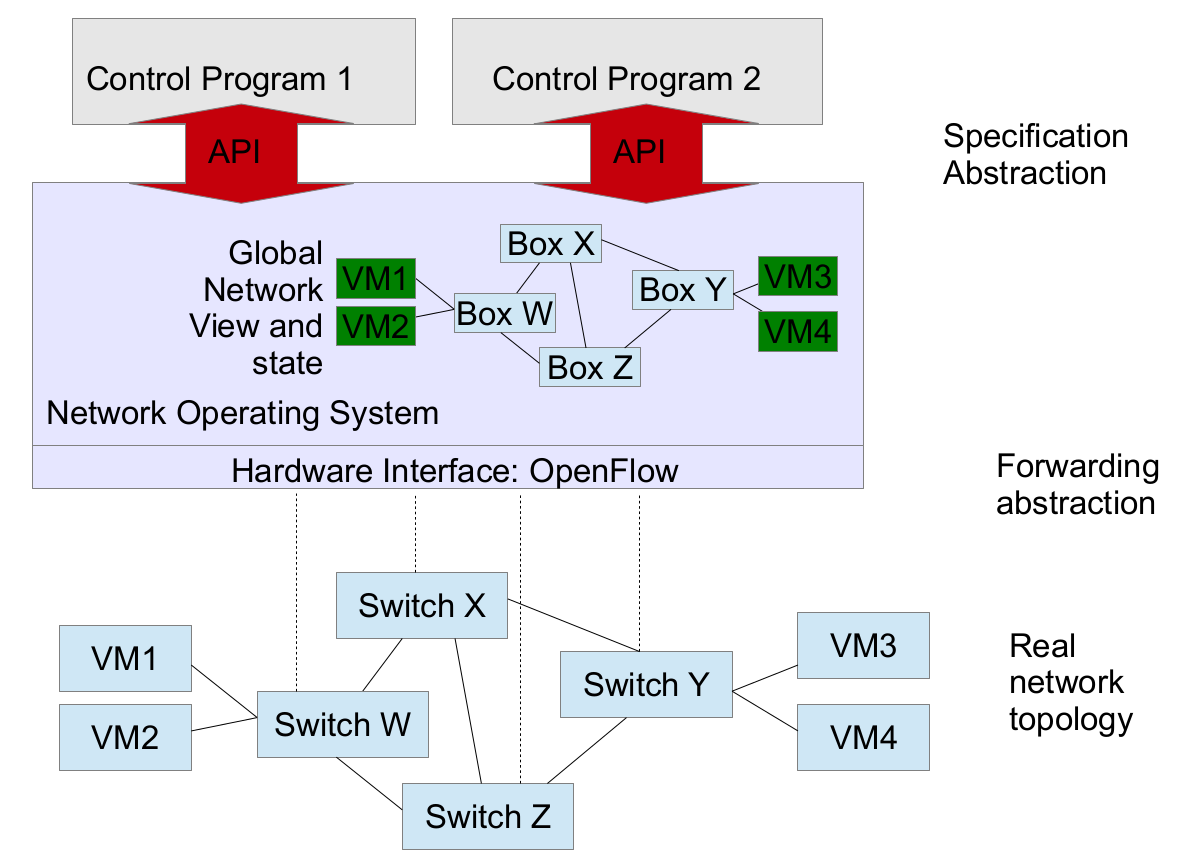
\includegraphics[width=.6\textwidth]{figures/network_operating_system.png}
  \caption{Network Operating System Model}\label{fig:network_operating_system}
\end{figure}
With an NOS we have a central control plane which handles the difficult network and routing computations.
This way the actual forwarding switches are only "dumb boxes" which are connected via ssl to the NOS which runs on fairly common CPUs.

Some disadvantages of SDN are that more configuration is required than in traditional forwarding and a single point of failure exists.
